\documentclass[11pt,letterpaper]{article}

% ---- base packages ----
\usepackage{graphicx}
\usepackage{xcolor}
\usepackage{geometry}
\usepackage{amsmath}
\usepackage{amssymb}
\usepackage{amsthm}
\usepackage{newtxtext}
\usepackage{newtxmath}
\usepackage{booktabs}
\usepackage{array}
\usepackage{enumitem}
\usepackage{microtype}
\usepackage{setspace}
\usepackage{caption}
\usepackage{fancyhdr}
\usepackage{tikz}
\usetikzlibrary{arrows.meta, positioning, shapes.geometric, calc}

% superscript numeric citations
\usepackage[numbers,super,sort&compress]{natbib}
\bibliographystyle{unsrtnat}

% hyperref LAST; hidden links (no colored text in the report)
\usepackage[
    hidelinks,
    bookmarks=true,
    bookmarksnumbered=true,
    unicode=true
]{hyperref}

% ---- STS formatting: 1in margins, 1.5 spacing, page numbers bottom right ----
\geometry{letterpaper, margin=1in}
\onehalfspacing
\emergencystretch=2em
\captionsetup{font=small, labelfont=bf, skip=4pt}
\setlist[itemize]{itemsep=0.2em, leftmargin=1.5em}
\AtBeginEnvironment{table}{\singlespacing}
\AtBeginEnvironment{figure}{\singlespacing}

\fancyhf{}
\renewcommand{\headrulewidth}{0pt}
\fancyfoot[R]{\thepage}
\pagestyle{fancy}

\hypersetup{
    pdftitle={When Does the Record of a Computation Matter?},
    pdfauthor={Sean Mahdavian},
    pdfsubject={Witness structure across substrates: proofs, edits, and circuits},
    pdfkeywords={witness supervision, process supervision, ZX calculus, Lean 4, quantum computing}
}

\newtheorem{definition}{Definition}
\newtheorem{theorem}{Theorem}
\newcommand{\simminus}{\mathrm{sim}-\mathrm{echo}}
\newcommand{\W}{\mathbf{W}}
\newcommand{\E}{\mathbf{E}}

\begin{document}

% ===================== TITLE PAGE (not counted) =====================
\thispagestyle{empty}
\begin{center}
\vspace*{2.2in}
{\LARGE\bfseries When Does the Record of a Computation Matter?\\[0.35em]}
{\large Witness structure across substrates: proofs, edits, and circuits\\[2.2em]}
{\large Sean Mahdavian\\[0.6em]}
{\normalsize Research Report (working draft)}
\vfill
\end{center}
\clearpage

% ===================== ABSTRACT PAGE (not counted) =====================
\thispagestyle{empty}
\begin{center}{\large\bfseries Abstract}\end{center}
\noindent
A transformation has endpoints and a record of how it was made.
Call that record the witness.
This paper asks when keeping the witness is worth it, and measures the answer on three substrates, the systems that carry a computation: gradient-descent training of a small language model (in two domains) and a superconducting quantum device.
The hypothesis under test: witness supervision pays exactly where the witness is not recoverable from the endpoints.
On 10{,}925 edits mined from Mathlib, a small language model trained with explicit diffs transfers no better than one trained with (before, after) endpoint pairs: the diff is cheap to recover from the endpoints, so writing it out adds nothing (Part~I).
On IBM \texttt{ibm\_fez}, four machine-verified ZX-optimized circuit pairs beat their baselines by up to $+0.067$ exact-answer probability, but the noise model's predicted ordering is wrong, and drift, routing, and dynamical-decoupling controls show the gain tracks circuit duration rather than gate counts (Part~II).
On LeanDojo tactic prediction, where recovering a proof step from its goal states is search, trace supervision beats endpoint pairing by $+0.024$ to $+0.050$ across three seeds, with 68 to 76\% of the gap from witness content rather than format exposure (Part~III).
The naive information-theoretic predictor of this contrast is the witness fiber, formalized in Lean and computed exactly.
It is provably wrong for the family tested.
Exact Bayes ceilings collapse at both ends of the fiber axis, so no monotone law from fiber size to the supervision gap can exist (Part~IV).
A budget sweep then shows the proof-step gap does not close across a $32\times$ range of endpoint data; the extrapolated zero-crossing sits near eight million examples, and the content share survives (Part~V).
A fourth predictor, an intermediate supervision channel whose exact ceilings \emph{are} monotone in the fiber, then fails its own registered test in the opposite direction (Spearman $-0.80$): available information does not predict used information (Part~VI).
A registered verification experiment stopped at its own anchor, so whether the advantage extends to checking witnesses is open at this scale.
I pre-registered all fifteen protocols with timestamped commits and recorded every verdict before interpretation; a public \texttt{verify.py} re-derives every table.
Trace supervision transfers something that endpoint data cannot buy at any budget tested, and the naive information-theoretic predictor of when this happens is provably wrong.
\clearpage

% ===================== BODY: page numbering starts here =====================
\setcounter{page}{1}

\section{Introduction}\label{sec:intro}

Every nontrivial computation produces two things: a pair of endpoints, an input and an output, and a record of how the second was obtained from the first. Call that record the \emph{witness}. In a proof it is the tactic sequence. In a refactor it is the diff. In a quantum computation it is the circuit that ran. Modern learning pipelines mostly keep the endpoints and discard the witness, on the quiet assumption that anything it could teach can be re-derived from the endpoints when needed. This paper asks when that assumption holds, and measures the answer on three substrates, the systems that carry a computation: gradient-descent training of a small language model, in two domains, and a superconducting quantum device.

The motivation is the search/verification asymmetry. For some transformations the witness is cheap to recover from the endpoints: the diff of two files is determined by them, up to a polynomial-time computation. For others, recovery is search: reconstructing the tactic that carries one Lean goal state to another means exploring a combinatorial space, while checking the tactic is cheap. If the endpoints determine the witness, supervising a model on the witness should add nothing to supervising it on the endpoints. If they do not, the witness carries information no endpoint pair can supply, and supervising on it should help. The ``if'' is the experiment: Part~I tests a domain where recovery is provably cheap, and Part~III tests one where recovery is search. One disclaimer belongs here: this asymmetry has the same shape as the definition of $\mathrm{NP}$, but the paper claims nothing about P versus NP. The asymmetry serves only to rank domains by recovery cost; nothing later should be read as evidence about complexity classes.

\begin{center}
\fbox{\parbox{0.94\textwidth}{\textbf{Hypothesis.} Supervision with the record pays exactly where the record is \emph{not} recoverable from the endpoints. Where recovery is cheap (code diffs), explicit witness supervision should add nothing over the endpoint pair. Where recovery is search (proof steps), it should transfer an advantage that endpoint data cannot supply at any budget.}}
\end{center}

The paper proceeds as follows. Section~\ref{sec:formal} defines the terms formally, in Lean: a witnessed transformation, the forgetful map to endpoint pairs, recoverability as faithfulness of that map, and the fiber as its quantitative version. These definitions do one job: they turn ``the witness adds something'' from an intuition into a quantity each experiment can measure. Part~I gives the null result: on Mathlib code edits, explicit diff supervision adds nothing once a metric error is repaired. Part~II gives the physical test: four machine-certified ZX circuit pairs on IBM \texttt{ibm\_fez} show a real, replicated fidelity gain, with the noise model's predicted ordering wrong and the mechanism shown to be duration, not gate count. Part~III gives the positive effect: on Lean tactic prediction, where measured gold-tactic recoverability is $0.003$, trace supervision wins by a large, content-dominated margin across three seeds. Part~IV gives the negative result: it tests the natural candidate law, that the gap grows with the witness fiber, and exact computation overturns it. The law is natural because more witnesses per endpoint pair means more hidden information; it still fails, because the evaluation's own ceilings cap any gap, and the ceilings are computable before any training runs. Part~V gives the mechanism: across a $32\times$ range of stage-2 budgets, the gap remains.

A second contribution is methodological. I pre-registered every experiment in a public repository before running it: fifteen protocols, each with explicit falsification clauses, each verdict timestamped before interpretation. Three designs stopped at their own registered checks, one of them twice, and all are reported as failures. One script, \texttt{verify.py}, re-derives every number in every table from committed artifacts~\cite{appliedrepo2026}.

\section{Background}\label{sec:background}

\paragraph{Certificates.} A decision problem is in $\mathrm{NP}$ when its yes-instances carry witnesses checkable in polynomial time. I use the find-versus-check gap only to choose domains; the paper proves no complexity result.

\paragraph{Lenses: backpropagation as keeping the record.} The categorical account of backpropagation models a supervised learner as a \emph{lens}: a forward map paired with a backward update, composed so that gradients flow through composites functorially~\cite{fong2019backprop,cruttwell2022categorical}. The backward pass is exactly the record: the computation keeps the trace of the forward sweep, so the update costs one backward pass instead of $2P$ forward passes (Figure~\ref{fig:lens}). Section~\ref{sec:formal} formalizes this in Lean and proves the seven laws that license treating a deep composite as a single lens.

\begin{figure}[htbp]
\centering
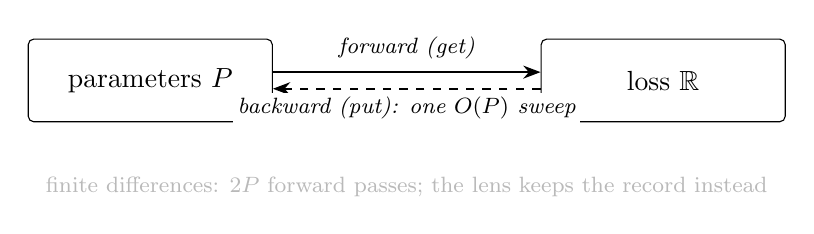
\begin{tikzpicture}[
    box/.style={draw, rounded corners=2pt, minimum width=3.1cm, minimum height=1.05cm, align=center},
    lbl/.style={font=\footnotesize\itshape},
    arr/.style={-{Stealth[length=2.2mm]}, thick}]
  \node[box] (A) {parameters $P$};
  \node[box, right=3.4cm of A] (B) {loss $\mathbb{R}$};
  \draw[arr] ([yshift=3pt]A.east) -- node[lbl, above=1pt]{forward (get)} ([yshift=3pt]B.west);
  \draw[arr, dashed] ([yshift=-3pt]B.west) -- node[lbl, below=1pt, fill=white, inner sep=1.5pt]{backward (put): one $O(P)$ sweep} ([yshift=-3pt]A.east);
  \node[font=\footnotesize, text=gray!55] at ($(A)!0.5!(B) + (0,-1.35)$) {finite differences: $2P$ forward passes; the lens keeps the record instead};
\end{tikzpicture}
\caption{A learner as a lens. The forward pass is the endpoints; the backward pass exists because the record of the forward sweep was kept. \emph{Source: figure created by the author.}}
\label{fig:lens}
\end{figure}

\paragraph{ZX calculus: circuits as diagrams, rewriting as compilation.} The ZX calculus represents quantum circuits as diagrams built from two kinds of nodes, called spiders, where each node is a linear map carrying a phase and each edge is a wire that contracts tensor indices. Rewriting the diagram, by spider fusion and the bialgebra (Frobenius) equations, is sound for linear-algebraic equality~\cite{coecke2011interacting}. Kissinger and van de Wetering showed that full diagrammatic reduction followed by circuit extraction cuts non-Clifford (T) counts substantially on standard benchmark suites, and released the method as PyZX's \texttt{full\_reduce}~\cite{kissinger2020reducing,kissinger2019pyzx}. The benchmark circuits come from the T-par and optimization literature~\cite{amy2014tpar,nam2018automated}. Part~II will ask hardware to trust this pipeline's output, so I first reran the pipeline end to end. It reproduces the published profile: a 46\% aggregate T-count reduction across the 30-circuit suite (6019 to 3253), within 3\% of the shipped T-par outputs head to head (2753 vs.\ 2829: five wins, eighteen ties, one loss), with a machine-checked equality witness for every circuit small enough to verify. That rerun is a reproduction with certificates, not a discovery, and the certificates are exactly what Part~II needs: every optimized circuit it ships must be provably the same computation as its baseline. Table~\ref{tab:tracka} gives representative rows; Figure~\ref{fig:zx} shows the pipeline on one pair.

\begin{table}[htbp]
\centering\footnotesize
\caption{Representative rows from the 30-circuit benchmark rerun (T-counts; \texttt{tpar} = published T-par outputs). Extraction after full reduction inflates two-qubit counts, so hardware runs use phase teleportation: same 46\% T-count win, two-qubit structure preserved, all witnesses green. \emph{Source: project data~\cite{appliedrepo2026}.}}
\label{tab:tracka}
\begin{tabular}{lccccc}
\toprule
circuit & qubits & T in & T out & T (T-par) & verified \\
\midrule
\texttt{mod5\_4} & 5 & 28 & \textbf{8} & 16 & PASS \\
\texttt{mod\_mult\_55} & 9 & 49 & \textbf{35} & 37 & PASS \\
\texttt{tof\_3} & 5 & 21 & 15 & 15 & PASS \\
\texttt{barenco\_tof\_3} & 5 & 28 & 16 & 16 & PASS \\
\bottomrule
\end{tabular}
\end{table}

\begin{figure}[htbp]
\centering
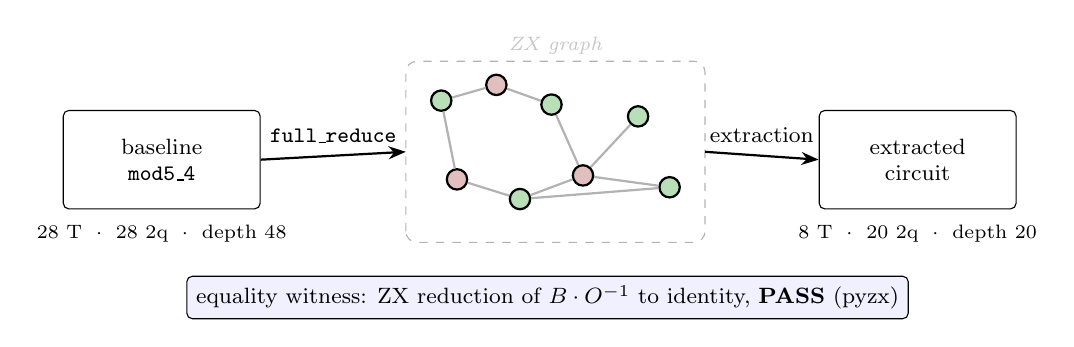
\begin{tikzpicture}[
    cbox/.style={draw, rounded corners=2pt, minimum width=2.5cm, minimum height=1.25cm, align=center, font=\footnotesize},
    zsp/.style={circle, draw, thick, fill=green!55!black!28, inner sep=2.6pt},
    xsp/.style={circle, draw, thick, fill=red!55!black!25, inner sep=2.6pt},
    wire/.style={thick, gray!60},
    arr/.style={-{Stealth[length=2.2mm]}, thick},
    lbl/.style={font=\footnotesize}]
  % baseline circuit
  \node[cbox] (base) at (0,0) {baseline\\ \texttt{mod5\_4}};
  \node[font=\scriptsize, below=2pt of base] {28 T\; $\cdot$\; 28 2q\; $\cdot$\; depth 48};
  % ZX graph panel
  \draw[rounded corners=4pt, dashed, gray!60] (3.1,-1.05) rectangle (6.9,1.25);
  \node[font=\scriptsize\itshape, gray!45] at (5.0,1.45) {ZX graph};
  \node[zsp] (g1) at (3.55,0.75) {};
  \node[xsp] (r1) at (4.25,0.95) {};
  \node[zsp] (g2) at (4.95,0.7) {};
  \node[xsp] (r2) at (3.75,-0.25) {};
  \node[zsp] (g3) at (4.55,-0.5) {};
  \node[xsp] (r3) at (5.35,-0.2) {};
  \node[zsp] (g4) at (6.05,0.55) {};
  \node[zsp] (g5) at (6.45,-0.35) {};
  \draw[wire] (g1)--(r1); \draw[wire] (r1)--(g2); \draw[wire] (g1)--(r2);
  \draw[wire] (r2)--(g3); \draw[wire] (g3)--(r3); \draw[wire] (r3)--(g4);
  \draw[wire] (g2)--(r3); \draw[wire] (r3)--(g5); \draw[wire] (g3)--(g5);
  % extracted circuit
  \node[cbox] (opt) at (9.6,0) {extracted\\ circuit};
  \node[font=\scriptsize, below=2pt of opt] {8 T\; $\cdot$\; 20 2q\; $\cdot$\; depth 20};
  % arrows
  \draw[arr] (base.east) -- node[lbl, above=1pt]{\texttt{full\_reduce}} (3.1,0.1);
  \draw[arr] (6.9,0.1) -- node[lbl, above=1pt]{extraction} (opt.west);
  % witness badge
  \node[draw, rounded corners=2pt, fill=blue!6, font=\footnotesize, align=center] at (4.9,-1.75)
    {equality witness: ZX reduction of $B\cdot O^{-1}$ to identity, \textbf{PASS} (pyzx)};
\end{tikzpicture}
\caption{Circuit $\to$ graph $\to$ smaller circuit, on the \texttt{mod5\_4} pair. Nodes are spiders (linear maps with phases), edges are wires; rewriting fuses connected spiders of the same color. The layout is schematic, the counts are not: they are the certified pre-transpile numbers of Part~II. \emph{Source: figure created by the author from project data~\cite{appliedrepo2026}.}}
\label{fig:zx}
\end{figure}

\paragraph{Process versus outcome supervision.} The distinction between supervising on intermediate steps and supervising on outcomes is well studied. Lightman et al.\ found process supervision substantially outperformed outcome supervision on competition mathematics, reaching 78\% on a MATH subset~\cite{lightman2023verify}; Uesato et al.\ reported related findings~\cite{uesato2022solving}. On the theory side, Jia, Rakhlin, and Xie prove that under standard coverage assumptions, outcome supervision is no more statistically difficult than process supervision up to polynomial factors in the horizon~\cite{jia2025verify}; any real gap is algorithmic, not an intrinsic statistical barrier. Parts~I and III rediscover a known phenomenon at small scale, and say so. The intended contribution is the controls: Part~I's metric repair, Part~III's shuffle and multi-seed controls, Part~V's mechanism test, and Part~IV's negative result.

\paragraph{Mirror circuits: the device checks itself.} Mirror circuits, which run a circuit followed by its inverse and check the return, were developed by Proctor and collaborators as a scalable benchmark of quantum computer capability~\cite{proctor2022measuring}. This project uses them as an application, not an invention: mirrors composed of a baseline circuit and its optimized partner make the hardware itself check the equality witnesses, with deranged (mismatched-pair) mirrors as a control against accidental returns (Section~\ref{sec:part2}).

Lenses, ZX diagrams, and mirror circuits are the vocabulary this paper needs. The next section puts the central distinction itself into formal form.

\section{The Formal Layer}\label{sec:formal}

When does keeping the record pay? Before experiment can answer, the question needs a precise object: a formal definition of the record, of what it means for the endpoints to determine it, and of how much it can carry. This section builds that object, and states exactly what the machine-checked layer does and does not do for the paper.

\subsection{Categorical preliminaries: the record as a morphism}\label{sec:prelim}

Start with states and the operations that change them. Fix a set $S$ of states and an alphabet $\mathrm{Op}$ of operations acting by $\mathrm{act}\colon \mathrm{Op}\times S\to S$. A \emph{witness} of length $L$ is a word $w=(o_1,\dots,o_L)\in\mathrm{Op}^L$; write $\mathrm{run}(w,s)$ for the iterated action. The witnessed transformations form a category $\W_L$: objects are states, a morphism $s\to t$ is a word $w$ with $\mathrm{run}(w,s)=t$, composition is concatenation, which is legal because $\mathrm{run}(w_1 w_2, s)=\mathrm{run}\!\bigl(w_2,\mathrm{run}(w_1,s)\bigr)$, and the identity is the empty word. Forgetting the word yields the \emph{endpoint category} $\E_L$ (same objects; a unique morphism $s\to t$ whenever some length-$L$ word runs $s$ to $t$) and a forgetful functor $U\colon \W_L\to\E_L$, the identity on objects and $w\mapsto(s,t)$ on morphisms.

\begin{definition}[Recoverability and the fiber]\label{def:fiber}
The system is \emph{recoverable} at $(s,L)$ when $U$ is faithful on morphisms out of $s$: any two length-$L$ words with the same action on $s$ are equal. The \emph{fiber} over an endpoint pair is the count $\varphi(s,t)=\bigl|U^{-1}(s\!\to\!t)\bigr|$ of length-$L$ words running $s$ to $t$. Recoverability is $\varphi\leq 1$ everywhere; otherwise $\log_2\varphi$ measures, in bits, the witness information the endpoints cannot supply.
\end{definition}

The supervision reading is immediate. When $\varphi=1$, the witness is a deterministic function of the endpoints, so any training signal it carries is already carried implicitly by the endpoint pair. Explicit witness supervision can then add nothing. Part~I's diffs are of this kind. When $\varphi>1$ and inversion is search, the witness carries information no endpoint pair supplies. Part~III's tactics are of this kind. Part~IV promotes $\varphi$ to a candidate predictor and refutes it on its own terms.

Two further structures support the gradient and hardware sides. \emph{Lenses.} A lens $(A,A')\rightleftarrows(B,B')$ is a pair $f\colon A\to B$ (forward) and $f'\colon A\times B'\to A'$ (backward); composition with $(g,g')$ has forward $g\circ f$ and backward $(a,c')\mapsto f'\bigl(a,\,g'(f(a),c')\bigr)$, so the backward pass of a composite decomposes through recorded intermediate values. This is exactly reverse-mode differentiation. \emph{Frobenius algebras.} A commutative Frobenius algebra $(A,\mu,\eta,\delta,\varepsilon)$ carries multiplication $\mu\colon A\otimes A\to A$ and comultiplication $\delta\colon A\to A\otimes A$ with (co)units, satisfying associativity and the Frobenius identity
\begin{equation}\label{eq:frob}
(\mathrm{id}\otimes\mu)\circ(\delta\otimes\mathrm{id}) \;=\; \delta\circ\mu \;=\; (\mu\otimes\mathrm{id})\circ(\mathrm{id}\otimes\delta).
\end{equation}
In the ZX calculus the two spider colors are two such algebras, fused by a bialgebra law; spider fusion is associativity, and every rewrite the compiler of Part~II applies is one of these equations. The companion Lean development formalizes the cobordism presentation $\mathrm{Cob}_2$ and its symmetric monoidal quotient, and proves the connected-spider composition law
\begin{equation}\label{eq:spider}
\mathrm{spider}(a,b,g)\circ \mathrm{spider}(b,c,h) \;=\; \mathrm{spider}\bigl(a,c,\; g+(b-1)+h\bigr),
\end{equation}
where $b$ is the shared boundary count and $g,h$ the genera~\cite{liquidtqft2026}. This is the equation that turns diagrammatic simplification from a heuristic into a certified compiler pass. With the objects in place, the rest of the section says what has been proved about them.

\subsection{What is machine-checked, and where}

Two Lean files and one companion repository carry the proofs. \texttt{LensLean.lean} (Mathlib-free) proves the seven category and monoidal laws for lenses: two identity laws, associativity, and four coherence equations. Every one is proved by \texttt{rfl}, which means the two sides are \emph{definitionally} equal: the categorical structure was already present in the definitions, not imposed on top. The laws matter operationally, because they license fusing a deep composite of lenses into one backward sweep. A companion benchmark (\texttt{bench\_lens.lean}) measures what the license buys: at 1024 components, one fused sweep against central finite differences separates by a factor of $10^6$, and the lens gradient matches the analytic gradient exactly (Table~\ref{tab:lensbench}).

\begin{table}[htbp]
\centering\footnotesize
\caption{One reverse-mode lens sweep vs.\ central finite differences, timed under the Lean interpreter on a degree-$P$ Horner polynomial (shapes meaningful, absolute values interpreter-bound). \emph{Source: project data~\cite{appliedrepo2026}.}}
\label{tab:lensbench}
\begin{tabular}{rccccc}
\toprule
$P$ & lens (ms) & FD (ms) & FD / lens & lens vs.\ analytic & FD vs.\ analytic \\
\midrule
8 & 0.00045 & 0.068 & 154 & 0.0 & 0.0 \\
256 & 0.00122 & 34.5 & 28{,}224 & 0.0 & $3\times10^{-6}$ \\
1024 & 0.00466 & 4{,}698 & 1{,}007{,}930 & 0.0 & $3\times10^{-6}$ \\
\bottomrule
\end{tabular}
\end{table}

\texttt{WitnessRecoverability.lean} formalizes Section~\ref{sec:prelim}'s axis. \texttt{free\_faithful} proves one end case: in the free system (states are stacks, operations push), the endpoint literally contains the witness, so $U$ is faithful at every length. Recovering the witness is reading. \texttt{abelian\_not\_faithful} proves the other end case: for two commuting bit flips, the two orderings are distinct witnesses with identical endpoints. The proof runs by kernel computation: \texttt{decide} evaluates the counterexample mechanically, with zero axioms. The counterexample is not argued; the kernel evaluates it. Part~IV's conditions interpolate between these two cases by mixing free and commuting generators, and \texttt{fiber.py} computes $\varphi$ for them by exhaustive enumeration, matching the Lean \texttt{\#eval} outputs on small systems. The companion repository holds the Frobenius side: the $\mathrm{Cob}_2$ presentation, its quotients, and \eqref{eq:spider}, all machine-checked against Mathlib v4.28.0~\cite{liquidtqft2026}.

\begin{table}[htbp]
\centering\footnotesize
\caption{The paper's informal notions, their formal objects, and where each is machine-checked.}
\label{tab:map}
\begin{tabular}{@{}lll@{}}
\toprule
informal notion & formal object & Lean file \\
\midrule
record of a computation & morphism of $\W_L$ & \texttt{WitnessRecoverability.lean} \\
``the record adds nothing'' & $U$ faithful ($\varphi = 1$) & \texttt{free\_faithful} \\
``the record carries bits'' & fiber $\varphi > 1$ & \texttt{abelian\_not\_faithful} (by \texttt{decide}) \\
compiler rewrite rule & Frobenius / spider equation & \texttt{Cob2*.lean}~\cite{liquidtqft2026} \\
gradient witness & lens composition laws & \texttt{LensLean.lean} \\
\bottomrule
\end{tabular}
\end{table}

\subsection{Axiom audit and provenance}

An audit with \texttt{\#print axioms} finds only \texttt{propext} and \texttt{Quot.sound} anywhere in the formal layer, Lean's standard logical infrastructure. There are no \texttt{sorry} placeholders and no custom axioms. Every theorem kernel-checks in seconds.

Provenance disclosure, stated here rather than buried: Claude (Anthropic) drafted the recoverability file and the ceiling derivation of Part~IV inside my categorical framework. I validated every definition, extended the file with the fiber layer and the demo computations, and I have rederived both proofs by hand. Lean proof search elsewhere in the broader program used Aristotle (Harmonic). I made every decision about what to formalize and every verdict call about what the formalization settles.

\subsection{What work the Lean actually does}\label{sec:leanwork}

Two concrete answers, both used later. First, the formal layer \emph{defines the axis}: the fiber of Section~\ref{sec:part4} is not a heuristic score but Definition~\ref{def:fiber}'s quantity, computed exactly. Second, its exact consequences \emph{stopped registered experiments}: the ceiling arithmetic of Section~\ref{sec:part4}, run before the full sweep, showed that design could not see the effect it was built to measure, and I stopped it after its sanity check; and the rank computation of Section~\ref{sec:secondneg} showed the conjectured endpoint-versus-trace gap cannot occur in these systems, stopping that design before registration. That is the work the Lean does: it made conjectures precise enough to refute cheaply.

\begin{figure}[htbp]
\centering
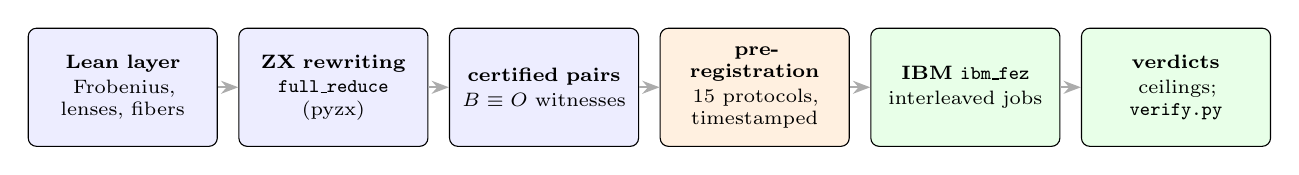
\begin{tikzpicture}[
    node distance=0.26cm,
    stage/.style={draw, rounded corners=3pt, align=center, font=\scriptsize, inner sep=4pt, text width=2.12cm, minimum height=1.5cm},
    arr/.style={-{Stealth[length=2.2mm]}, thick, gray!65}]
  \node[stage, fill=blue!7] (lean) {\textbf{Lean layer}\\[1pt] Frobenius, lenses, fibers};
  \node[stage, fill=blue!7, right=of lean] (pyzx) {\textbf{ZX rewriting}\\[1pt] \texttt{full\_reduce} (pyzx)};
  \node[stage, fill=blue!7, right=of pyzx] (cert) {\textbf{certified pairs}\\[1pt] $B\equiv O$ witnesses};
  \node[stage, fill=orange!12, right=of cert] (prereg) {\textbf{pre-registration}\\[1pt] 15 protocols, timestamped};
  \node[stage, fill=green!9, right=of prereg] (hw) {\textbf{IBM \texttt{ibm\_fez}}\\[1pt] interleaved jobs};
  \node[stage, fill=green!9, right=of hw] (verdict) {\textbf{verdicts}\\[1pt] ceilings; \texttt{verify.py}};
  \draw[arr] (lean) -- (pyzx);
  \draw[arr] (pyzx) -- (cert);
  \draw[arr] (cert) -- (prereg);
  \draw[arr] (prereg) -- (hw);
  \draw[arr] (hw) -- (verdict);
\end{tikzpicture}
\caption{Provenance chain, redrawn from the repository. Every hardware number descends from a machine-checked equality witness and a pre-registered prediction; \texttt{verify.py} re-derives every table from committed artifacts. \emph{Source: figure created by the author.}}
\label{fig:provenance}
\end{figure}

\section{Part I: Code Edits, Where the Record Is Cheap}\label{sec:part1}

\subsection{Design}

The cheap-recovery case is the code edit: given the before and after states, computing the diff is a polynomial-time operation. If the recoverability hypothesis is right, supervising a model on the explicit diff should add nothing over supervising on the endpoint pair. The original protocol registered four predictions: P1, a diff-trained arm shows a zero-shot lead when asked to predict edits; P2, the headline, a durable advantage after a small shared adaptation; P3, a null on a control comparison; P4, protocol hygiene on both ends.

I mined 10{,}925 single-file edit records from the most recent 20{,}000 commits of the community \texttt{mathlib4} repository (shallow clone, 2026-07-18), sorted them by date, and held out the final 5\%; evaluation scores the first 300 held-out items. The model is Pythia-410M with LoRA adapters (rank 16), bf16 on a GB10, seed 0~\cite{biderman2023pythia}. Stage~1 trains three arms on identical data, budget (20M tokens each), and seed. Only the format differs: \texttt{ck\_diff} sees \textsc{before} + \textsc{diff} (the record), \texttt{ck\_after} sees \textsc{before} + \textsc{after} (the endpoint pair), \texttt{ck\_endpoint} sees \textsc{after} alone. Stage~2 adapts each checkpoint on the same small diff-format dose (1M tokens), giving \texttt{ad\_diff}, \texttt{ad\_after}, \texttt{ad\_endpoint}. The question: which stage-1 supervision best supports the shared downstream task of predicting edits?

\subsection{The metric error, first-class}

The v1 run returned an apparent confirmation that a skeptical second read took apart, and that correction matters as much as anything that remained. The v1 metric, mean character similarity to the gold diff, rewards echoing the before-window, because a diff mostly repeats its context. Every adapted arm scored at the context-echo ceiling ($\approx 0.243$), indistinguishable on actual edit content; v1 also saved means rather than per-item scores, blocking audit after the fact. The repair is the \emph{echo ceiling}: for each item, score the similarity of the before-window itself to the gold diff, which is what pure copying earns, and report $\simminus$, the per-item difference. Copying scores zero by construction. The repair removed the original claim. Pre-registration plus the audit habit caught the error, and I report both the failure and the fix rather than editing them away.

\subsection{Results}

The v2 suite scores every checkpoint per item on six measures: raw similarity (the v1 metric, kept for continuity), edit-line-only similarity, the echo ceiling, $\simminus$, applicability (does the generation's implied pre-image occur contiguously in the before-window), and implied-after similarity, which resists echo. Table~\ref{tab:part1full} gives the headline metrics; Table~\ref{tab:part1} gives the surviving paired comparisons, recomputed independently by \texttt{verify.py} from the committed per-item scores (paired Wilcoxon signed-rank, $n = 300$).

\begin{table}[htbp]
\centering\footnotesize
\caption{Part I metric suite, all six checkpoints (seed 0, $n = 300$). The echo ceiling is identical across arms by construction; every arm scores below it on raw similarity, which confirms the v1 error a second time. The full six-metric suite is committed in the repository. \emph{Source: project data~\cite{appliedrepo2026}.}}
\label{tab:part1full}
\begin{tabular}{lcccc}
\toprule
arm & sim (v1) & echo & $\simminus$ & applies \\
\midrule
\texttt{ck\_diff} & 0.2311 & 0.2636 & $-0.033$ & 7.7\% \\
\texttt{ck\_after} & 0.1455 & 0.2636 & $-0.118$ & 6.3\% \\
\texttt{ck\_endpoint} & 0.0887 & 0.2636 & $-0.175$ & 0.7\% \\
\texttt{ad\_diff} & 0.2184 & 0.2636 & $-0.045$ & 9.7\% \\
\texttt{ad\_after} & 0.2046 & 0.2636 & $-0.059$ & 8.0\% \\
\texttt{ad\_endpoint} & 0.1706 & 0.2636 & $-0.093$ & 5.3\% \\
\bottomrule
\end{tabular}
\end{table}

\begin{table}[htbp]
\centering\small
\caption{Part I surviving results (v2 metrics, seed 0, $n=300$). The headline comparison is a null; both paired-format arms beat the endpoint-only arm decisively. \emph{Source: project data~\cite{appliedrepo2026}.}}
\label{tab:part1}
\begin{tabular}{lllcl}
\toprule
comparison & metric & mean $\Delta$ & wins to losses & $p$ \\
\midrule
\texttt{ad\_diff} $-$ \texttt{ad\_after} & $\simminus$ & $+0.014$ & 159 to 140 & $0.152$ \\
\texttt{ad\_diff} $-$ \texttt{ad\_endpoint} & $\simminus$ & $+0.048$ & 187 to 113 & $1.6\times10^{-5}$ \\
\texttt{ad\_after} $-$ \texttt{ad\_endpoint} & $\simminus$ & $+0.034$ & 184 to 116 & $2.4\times10^{-4}$ \\
\bottomrule
\end{tabular}
\end{table}

The bootstrap 95\% interval for the headline is $[-0.006, +0.034]$, which includes zero. The pattern is consistent across the artifact-proof metrics: the two paired-format arms are statistically indistinguishable from each other and both sit clearly above the endpoint-only arm. For edit-line similarity the diff arm holds a marginal lead ($p = 0.063$, interval $[+0.002, +0.042]$), the one thread a seed-1 run would settle.

Two secondary observations sharpen the picture. Zero-shot, the record arm's lead is real edit content: \texttt{ck\_diff} emits at least one edit line on 95\% of items, against 8\% and 18\% for the pair and endpoint arms, replicating at full $n$ the five-sample autopsy that flagged the effect in v1. After adaptation, the endpoint arm's behavior is diagnostic: it over-produces edit lines (mean 18.2 per item) with a 5\% applicable rate. That is format without content.

\subsection{Verdict}

P1 confirmed again: the zero-shot lead is genuine edit content, not echo. P2, strong form (explicit diff format beats paired endpoints): not supported; after identical adaptation the two arms are indistinguishable. P2, weak form (paired path structure beats endpoint-only): strongly supported, on every artifact-proof metric. Pairing transfers; serialization does not. Training on \textsc{before} + \textsc{after}, which keeps both states of the transformation in context, transfers to diff prediction statistically indistinguishably from training on the explicit diff. Removing the before-state is decisively harmful. This is exactly what recoverability predicts: the diff is recoverable from the endpoints, so writing it out adds nothing. In the program's framing: keep the section, not its integral. The section turns out to be the (before, after) pair itself, and the explicit diff is one way of writing it down, not a privileged form.

One note on independence: v1 ran remotely (fp32, T4); this run rebuilt the pipeline locally (bf16, GB10) with one day of commit drift, an independent draw that reached the same verdict on the repaired metric.

\medskip
\noindent\emph{Limitations carried forward.} Single training seed; 410M scale; one-day commit drift against the v1 window; results specific to Mathlib-style single-file edits.

\section{Part II: Quantum Circuits on Hardware}\label{sec:part2}

\subsection{Design}

Part~II moves the question to a physical substrate. I took four circuit pairs (\texttt{mod5\_4}, \texttt{tof\_3}, \texttt{barenco\_tof\_3}, \texttt{mod\_mult\_55}) from the Amy--Maslov--Nam benchmark family~\cite{amy2014tpar,nam2018automated}. Each pair implements one unitary twice: the standard baseline and a ZX-rewritten optimized circuit. ZX reduction machine-verifies pair equality before shipping (all four PASS), and \texttt{verify.py} re-verifies it independently from the committed QASM (Table~\ref{tab:pairs}). The record here is the compilation history: the rewrite proof that certifies the optimized circuit \emph{is} the same computation. I registered the predictions before any hardware ran, under a 1\% two-qubit depolarizing model, in size order: \texttt{mod5\_4} $+0.048$ $>$ \texttt{mod\_mult\_55} $+0.029$ $>$ \texttt{barenco\_tof\_3} $+0.020$ $>$ \texttt{tof\_3} $+0.013$ (near-parity control). Execution as registered: both arms interleaved in one job per pair, 8192 shots per arm, optimization level 1, \texttt{seed\_transpiler\,=\,7}, IBM \texttt{ibm\_fez}, 2026-07-18~\cite{javadi2024qiskit}. A noiseless simulator check ran first (both arms fidelity 1.0, delta zero), so any gap on the chip is hardware, not a compile error. One note on the metric: all four circuits have deterministic ideal outputs, a single bitstring, so ``fidelity'' here means the probability of measuring the exact correct answer. The layout pass placed all four pairs on overlapping low-error subsets in the qubit 117 to 145 region (mean CZ error $1.85$ to $2.11\times10^{-3}$ on the edges used, below that day's median).

\begin{table}[htbp]
\centering\small
\caption{Certified pairs, pre-transpile counts (baseline $\to$ optimized). Verification: ZX reduction of the composed pair to the identity. \emph{Source: project data~\cite{appliedrepo2026}.}}
\label{tab:pairs}
\begin{tabular}{lccccc}
\toprule
circuit & qubits & 2q gates & T-count & depth & verified \\
\midrule
\texttt{mod5\_4} & 5 & $28 \to 20$ & $28 \to 8$ & $48 \to 20$ & PASS \\
\texttt{tof\_3} & 5 & $18 \to 16$ & $21 \to 15$ & $31 \to 30$ & PASS \\
\texttt{barenco\_tof\_3} & 5 & $24 \to 22$ & $28 \to 16$ & $42 \to 43$ & PASS \\
\texttt{mod\_mult\_55} & 9 & $48 \to 42$ & $49 \to 35$ & $51 \to 46$ & PASS \\
\bottomrule
\end{tabular}
\end{table}

\subsection{Results}

\begin{table}[htbp]
\centering\small
\caption{Part II main results, IBM \texttt{ibm\_fez}, 2026-07-18. $z$ from per-shot paired statistics; transpiled counts are post-layout. \emph{Source: project data~\cite{appliedrepo2026}.}}
\label{tab:part2}
\begin{tabular}{lccccc}
\toprule
pair & $\Delta$ observed & $z$ & $\Delta$ predicted & transpiled 2q (b$\to$o) & depth (b$\to$o) \\
\midrule
\texttt{mod\_mult\_55} & $+0.0670$ & $+9.5$ & $+0.029$ & $99 \to 117$ & $217 \to 204$ \\
\texttt{mod5\_4} & $+0.0248$ & $+4.8$ & $+0.048$ & $52 \to 38$ & $206 \to 95$ \\
\texttt{barenco\_tof\_3} & $+0.0167$ & $+3.9$ & $+0.020$ & $42 \to 34$ & $164 \to 126$ \\
\texttt{tof\_3} (control) & $-0.0042$ & $-1.1$ & $+0.013$ & $30 \to 28$ & $118 \to 112$ \\
\bottomrule
\end{tabular}
\end{table}

Two verdicts, per the registered decision tree. \emph{Direction: confirmed} on all three effect pairs. The control landed at $-0.004$, within shot noise of zero, which rules out a systematic interleaved-arm bias. \emph{Ordering: falsified}, and stated as falsified. The registered ladder put \texttt{mod5\_4} first and \texttt{mod\_mult\_55} second; observation inverted them. The 9-qubit circuit won by the largest margin despite carrying \emph{more} transpiled two-qubit gates than its baseline (117 vs.\ 99). It won through depth (204 vs.\ 217): on a real device, coherence time prices circuits alongside gate error, so a one-parameter depolarizing model cannot rank them. Compilation pays on hardware; the simulator's ordering does not transfer.

\begin{figure}[htbp]
\centering
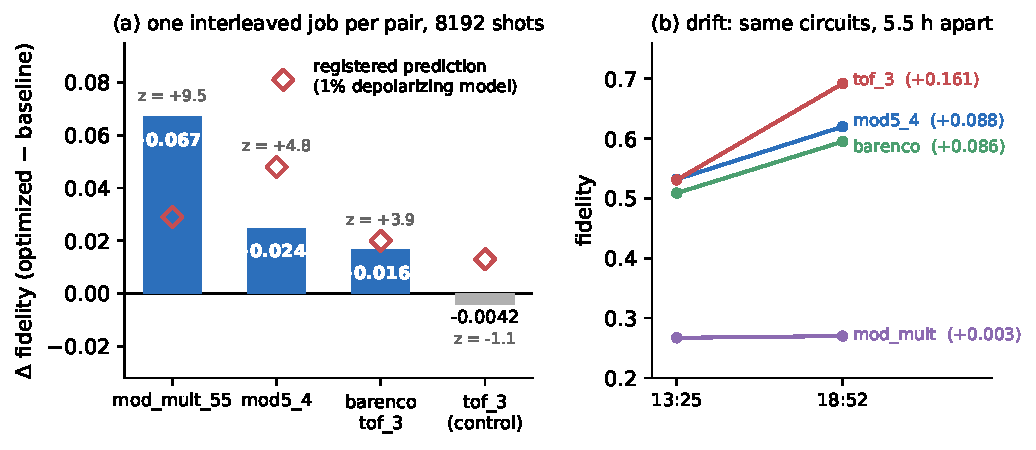
\includegraphics[width=0.92\textwidth]{figs/f3_part2_deltas.pdf}
\caption{Part II results in two panels. (a) Observed deltas against the registered predictions, one interleaved job per pair, 8192 shots, IBM \texttt{ibm\_fez}, 2026-07-18. (b) The drift measurement behind the interleaving rule: identical circuits in identical no-DD condition, re-measured hours later, move by up to $+0.161$. \emph{Source: figure created by the author from project data~\cite{appliedrepo2026}.}}
\label{fig:part2}
\end{figure}

\subsection{Error budget against the device ceiling}

After the verdict (not pre-registered), I compared each arm against its ceiling from that day's recovered calibration: $\prod(1-\varepsilon_{\mathrm{CZ}})$ over the exact edges used, times $\prod(1-\varepsilon_{\mathrm{ro}})$ over the exact qubits measured (Table~\ref{tab:ceilinghw}). Seven of eight arms sit at 99\% to 104\% of ceiling: the runs saturate the unmitigated hardware limit, so the deltas are close to a pure compilation effect. The one sub-ceiling arm, the \texttt{mod\_mult\_55} baseline at 89\%, carries about eight points of error the gate-count model cannot explain, while its optimized arm on mostly the same qubits sits at 103\%. The excess tracks circuit duration, independently supporting the duration reading. Above-ceiling values are physical: randomized benchmarking counts all Pauli errors~\cite{magesan2012rb}, but Z-type errors near measurement do not change a computational-basis output, so the RB ceiling is mildly conservative for this family.

\begin{table}[htbp]
\centering\small
\caption{Error budget vs.\ execution-time calibration (recovered from the four jobs' backend properties). Above-ceiling values are physical for this circuit family (see text). \emph{Source: project data~\cite{appliedrepo2026}.}}
\label{tab:ceilinghw}
\begin{tabular}{llccc}
\toprule
pair & arm & ceiling & measured & \% of ceiling \\
\midrule
\texttt{mod5\_4} & baseline & 0.875 & 0.865 & 99\% \\
\texttt{mod5\_4} & optimized & 0.902 & 0.890 & 99\% \\
\texttt{tof\_3} & baseline & 0.908 & 0.941 & 104\% \\
\texttt{tof\_3} & optimized & 0.913 & 0.937 & 103\% \\
\texttt{barenco\_tof\_3} & baseline & 0.892 & 0.912 & 102\% \\
\texttt{barenco\_tof\_3} & optimized & 0.907 & 0.928 & 102\% \\
\texttt{mod\_mult\_55} & baseline & 0.758 & 0.678 & \textbf{89\%} \\
\texttt{mod\_mult\_55} & optimized & 0.726 & 0.745 & 103\% \\
\bottomrule
\end{tabular}
\end{table}

One further covariate qualifies the registered number. A transpile-seed sweep (20 seeds, level 1, Fez snapshot) shows seed~7 gave the \texttt{mod\_mult\_55} optimized arm its \emph{worst} routing of all twenty (117 2q; sweep minimum 102, median 112.5), while the baseline drew near-best routing (99; minimum 96). The registered $+0.067$ was therefore measured with the optimized arm at its worst draw, and is plausibly a lower bound on the compilation effect at this site.

\subsection{Replication, routing decomposition, and drift}

Six days later I re-ran the flagship pair under stricter control (R2$'$): both arms pinned to one shared nine-qubit layout, one interleaved job. Baseline 99 2q at fidelity 0.639; optimized 102 2q at 0.700. The delta, $+0.0604$ against the registered $+0.0670$, shows the compilation gain replicates at matched placement. A third arm on identical qubits with deliberately worse routing (114 2q) measured 0.565: a routing effect of $-0.1346$ for 12 extra two-qubit gates and 18 extra depth. With that day's calibration (mean CZ $5.38\times10^{-3}$ vs.\ $4.63\times10^{-3}$ on the good edges), the ceiling model explains 0.077 of the 0.135 drop: 57\%, the corrected figure, superseding an earlier informal 5$\times$ estimate that used the wrong CZ error. The remaining $\approx 0.058$ tracks depth. Routing skill matters, but depth has its own measurable price.

The device state that day is part of the record: CZ errors on these qubits ran $4.48$ to $5.38\times10^{-3}$, more than double the $2.11\times10^{-3}$ of 2026-07-18, and all three arms beat their ceilings (107\%, 121\%, 112\%), consistent with RB conservatism for computational-basis outputs.

The drift measurement justifies the interleaving rule. Same circuits, same no-DD condition, two jobs 5.5 hours apart: \texttt{mod5\_4} $0.532 \to 0.620$; \texttt{tof\_3} $0.531 \to 0.692$; \texttt{barenco} $0.509 \to 0.595$; \texttt{mod\_mult} $0.267 \to 0.270$. That is up to $+0.161$ in an afternoon, and $+0.03$ to $+0.08$ in the 32 minutes between two consecutive jobs. These swings exceed most effects measured in this project, including the registered $+0.067$. Any cross-job comparison in this work is therefore uninterpretable, which is why the cross-job DD comparison (R1) is invalid as executed.

\subsection{The mirror protocol, dynamical decoupling, and two rejected explanations}

The mirror experiment makes the hardware itself check the equality witnesses. For each registered pair $p$, a \emph{true mirror} runs $X(x)\cdot B_p \cdot O_p^{-1}$ on a random input basis state $|x\rangle$ (seeded, recorded), with barriers so the transpiler cannot cancel the halves; if $B_p \equiv O_p$ the composition returns exactly $x$. A \emph{deranged mirror} runs $X(x)\cdot B_p \cdot O_q^{-1}$ with $q \neq p$, and $x$ is redrawn until the ideal output differs from $x$, which guards against inputs that happen to be fixed points of the composition. The metric is the return probability $r = P(\text{measure exactly } x)$ at 8192 shots, all circuits in one interleaved job. Registered predictions: M1, every true mirror returns $r \geq 0.25$ and beats its deranged partner by 0.3; M2, point predictions from the product of the per-arm fidelities ($\pm 0.15$); M3, every deranged mirror stays at $r \leq 0.15$. One honest design note belongs in the record: the first draft placed a random Pauli layer at the joint, which is wrong for non-Clifford circuits (the layer conjugates through $B$, so the expected string would need simulation, defeating the protocol). Randomized inputs give the same protection with a simulation-free expectation; the correction was logged before submission.

Results. True mirrors returned 0.267 to 0.692; deranged mirrors 0.0002 to 0.086. M3 confirmed; the derangement control works. The M2 point predictions failed low on all four pairs. Two hypotheses were registered to explain the undershoot: idle dephasing (suppressing it should raise true-mirror returns) and metric blindness (per-arm fidelity is scored on computational-basis histograms, blind to the phase errors a mirror exposes through $O^{-1}$).

The first test of idle dephasing (R1) compared separate jobs five hours apart and is confounded by drift; Section~\ref{sec:errors} owns that design error in full, and its recorded verdicts (R1a/b failed, R1c confirmed) stand as measured but isolate nothing.

The corrected rerun (R1$'$) put all sixteen circuits, eight mirrors times \{no-DD, DD\}, in one job, with DD as an XX sequence of native X pulses. Result: uniformly harmful. Paired deltas $-0.076$, $-0.022$, $-0.005$, $-0.039$, mean $-0.036$. Deranged mirrors stayed under 0.15 as registered (max 0.070), so DD did not manufacture signal. The added pulses, 80 to 225 per circuit, cost more error than the idle dephasing they suppress at this scale. Per the falsification clause, the idle-dephasing explanation is \textbf{rejected}. The metric-blindness hypothesis remains \textbf{untested} by any run so far, and I label it as such rather than carry it quietly. One data-integrity caveat: DD pads idle qubits across the full 156-qubit register, so the extraction step counts every qubit and the recorded DD-arm ceilings collapse to 0.039. They are artifacts; only the no-DD ceilings are used.

\subsection{Two design errors, owned}\label{sec:errors}

\paragraph{Cross-job DD (R1).} The first DD run compared a DD job at 13:25 against a no-DD job at 18:20: five hours of device drift confounded with the treatment, in direct violation of this project's own interleaving protocol. Its measured deltas were mixed in sign (\texttt{mod5\_4} $-0.033$, \texttt{tof\_3} $+0.089$, \texttt{barenco} $+0.055$, \texttt{mod\_mult\_55} $-0.115$; mean $-0.001$; deranged max 0.086), so R1a/b failed and R1c confirmed, and the recorded verdicts stand as measured. But the run does not isolate a DD effect; two of its four sign readings were later shown to be drift. R1$'$ is the corrected measurement.

\paragraph{Seed changes layout (R2).} The seed-11 rerun treated \texttt{seed\_transpiler} as a routing knob. It is not: the seed changes the layout, and the two arms landed on disjoint physical qubits (0/9 overlap, versus 7/9 in the registered runs). Its $+0.171$ delta therefore compared two different qubit sets and is not comparable to the registered $+0.067$. R2$'$ is the corrected measurement, and the seed sweep that exposed the error is committed alongside it.

\section{Part III: Proof Steps, Where Recovery Is Search}\label{sec:part3}

\subsection{From Part I to Part III}

Part~I's null says explicit record supervision adds nothing where the record is determined by the endpoints. The measured diagnostic for the other end: in the proof-step domain, the fraction of gold tactics appearing anywhere as a substring of the concatenated input states is $0.003$. Diffs in Part~I are fully determined by their endpoints; tactics are, for practical purposes, absent from them. Checking a tactic is cheap, since Lean's kernel does it, but reconstructing one from the goal states is search. If recoverability is the variable, this is where trace supervision should pay.

\subsection{Design}

Data: LeanDojo benchmark 4, mathlib4 tactic steps, split by theorem name so no held-out theorem leaks into training~\cite{yang2023leandojo}. Model: Pythia-160M, fp32, seed 0 for the registered run and seeds 1 and 2 as replicates~\cite{biderman2023pythia}. Three stage-1 corpora at matched token budget: \texttt{pw\_trace} (state-before + tactic + state-after, the full record), \texttt{pw\_pair} (the two endpoint states), \texttt{pw\_endpoint} (the after-state alone). Stage~2 is an identical small fine-tune for every arm on the eval format: given both states, predict the tactic. Metrics: exact match, normalized similarity, and $\simminus$ as repaired in Part~I. I registered three predictions. P1: \texttt{pw\_trace} beats \texttt{pw\_pair} on $\simminus$ (paired Wilcoxon $p<0.05$, mean $\geq +0.02$), the registered \emph{reversal} of Part~I's null. P2: \texttt{pw\_pair} beats \texttt{pw\_endpoint}. P3, the falsification branch: a \texttt{pw\_trace} $\approx$ \texttt{pw\_pair} tie would drop the complexity framing from the writeup, not soften it. A registered addendum added the format-exposure control: \texttt{pw\_shuffle} trains on \textsc{before} + a real but \emph{wrong} tactic (a derangement over training steps) + \textsc{after}, so it sees tactic-format text with no valid content. C1: \texttt{pw\_trace} beats \texttt{pw\_shuffle}, meaning the gain is witness content. C2: \texttt{pw\_shuffle} vs.\ \texttt{pw\_pair}, reported as observed.

\subsection{Results across three seeds}

\begin{table}[htbp]
\centering\footnotesize
\caption{Part III, multi-seed replication. The headline is the range, not a point estimate. \emph{Source: project data~\cite{appliedrepo2026}.}}
\label{tab:part3}
\begin{tabular}{lccc}
\toprule
 & seed 0 & seed 1 & seed 2 \\
\midrule
C1: trace $-$ shuffle & $+0.0393$ ($p = 1.4\!\times\!10^{-5}$) & $+0.0500$ ($p = 3.3\!\times\!10^{-9}$) & $+0.0240$ ($p = 0.0055$) \\
C2: shuffle $-$ pair & \multicolumn{3}{c}{mean $+0.0122$, all $p < 0.05$} \\
P2: pair $-$ endpoint & \multicolumn{3}{c}{null in all seeds ($p = 0.60,\ 0.28,\ 0.77$)} \\
\bottomrule
\end{tabular}
\end{table}

At the registered seed, P1 confirmed at $+0.0540$ (202 to 87, $p = 3.4\times10^{-13}$). The multi-seed round registered three checks before running: R3a, C1 stays positive with $p < 0.05$ in every seed; R3b, the across-seed standard deviation of the C1 mean delta stays below 0.02; R3c, P2 remains null in every seed. All three confirmed. C1 holds at $+0.0393$, $+0.0500$, $+0.0240$ across seeds 0, 1, 2 (sd 0.0131); C2 averages $+0.0122$ (sd 0.0046), significant in every seed; P2 stays null ($p = 0.60$, $0.28$, $0.77$). But the C1 magnitude ranges from $+0.024$ to $+0.050$, a factor of two. Sign and significance are robust; magnitude is not, so the range is the reported quantity. The decomposition is stable: content (C1) dominates format (C2), with content share 76\% across seeds (73\% at the Part~III operating point, $N = 2000$ stage-2 examples).

\subsection{Honest limitation, and a logged deviation}

All arms score below the copy baseline in absolute terms: $\simminus$ is negative throughout, because at 160M parameters the model cannot actually do tactic prediction. Every comparison in this section is therefore a valid comparison \emph{among models that cannot perform the task}. The effect is real, paired, replicated, and content-dominated, and it lives in a regime where the absolute capability is zero. Larger models are untested.

One protocol deviation is logged in the repository and belongs in the paper: the first registered training run diverged (loss spike, unrecovered). Per the registration's deviation rule, I committed the fix (a lowered stage-1 learning rate, $5\!\times\!10^{-5}$, unchanged across arms) and the rerun with dated notes before any evaluation ran. Every number reported here comes from the rerun.

\subsection{The tautology objection}

Isn't ``training on tactics helps predict tactics'' a tautology? Three registered controls stand between the claim and that objection. Stage~2 equalizes task exposure: every arm receives the identical fine-tune on the identical eval format, so all arms have seen what the task \emph{is}. The shuffle arm equalizes format: it too saw tactic-shaped text in stage~1, and it loses to the trace arm by the full C1 margin. Seeing the format is not what transfers. What remains is content, and Part~V shows volume does not equalize that either: $32\times$ more stage-2 examples do not close the gap.

\section{Part IV: The Formalized, Falsified Predictor}\label{sec:part4}

Parts I and III found opposite results in two domains. The obvious candidate law says the difference is quantitative: the supervision gap grows with the witness fiber, Definition~\ref{def:fiber}'s count, formalized in Lean. Part~IV formalized that law, pre-registered it, and refuted it.

\subsection{The registered design}

Six conditions, each a system of eight operations on a 28-bit state with witness length $L = 6$. Vocabulary, witness length, state representation, output length, and operation names are identical across conditions; names are opaque (\texttt{OP0}\dots\texttt{OP7}) so no structure leaks through labels. Only the algebra differs, interpolating between the two end cases proved in Section~\ref{sec:formal}. I computed fiber sizes \emph{exactly}, by full enumeration of all $8^6 = 262{,}144$ witnesses per condition: readable 1.0, free 1.0, q25 2.8, q50 29.7, q75 349.1, abelian 2581.0. Four arms per condition (trace / pair / endpoint / shuffle) at matched character budget, trained under the Part~III protocol (Pythia-160M, fp32, stage-1 lr $5\times10^{-5}$, stage-2 lr $2\times10^{-5}$, seed 0 registered, seeds 1 and 2 as replicates): 24 training runs in total. The eval asks the model to generate the witness from the endpoint pair; the primary metric is token accuracy over the six operation slots, chance $= 0.125$. The witness alphabet is disjoint from the state alphabet, so copying the input cannot beat chance and no echo correction is required. Registered predictions: P4a, the gap grows with $\log_2$ fiber (slope $>0$, $p<0.05$, $r^2 \geq 0.5$); P4b, \texttt{free} exceeds \texttt{readable} by $\geq 0.05$ (same fiber, opposite invertibility); P4c, the sanity anchor: on \texttt{readable}, where the end state literally contains the witness, all arms exceed 0.80 and the gap is below 0.05; P4d, content share above 50\% in the high-fiber conditions.

\subsection{The failed sanity check}

P4c failed on the first condition. Every arm scored at chance, 0.121 to 0.161 against a chance level of 0.125, because the state was rendered as a binary string and the model could not decode nibbles. The registration said that if the sanity anchor fails, no other prediction in the file may be interpreted. I stopped the sweep after one condition, on the registered rule.

\subsection{The computation that retired the design}

Working through the failure exposed something deeper than the encoding. The gap must vanish at \emph{both} ends of the fiber axis. At fiber 1 with an easy encoding, the inverse is learnable and stage~2 alone teaches both arms, so the low end fails. At large fiber, the witness is not determined by the endpoints, so \emph{no} arm can exceed a near-chance ceiling, and the high end fails. Table~\ref{tab:ceiling} makes this exact: Bayes ceilings by full enumeration, and the maximum possible gap (ceiling minus chance) at each condition.

\begin{table}[htbp]
\centering\footnotesize
\caption{Exact Bayes ceilings (generation-from-endpoints eval, $L = 6$). The maximum gap any supervision format could produce collapses at both ends of the fiber axis. \emph{Source: project data~\cite{appliedrepo2026}.}}
\label{tab:ceiling}
\begin{tabular}{lccc}
\toprule
condition & mean fiber & Bayes ceiling & max gap \\
\midrule
readable & 1.0 & 1.000 & 0.875 \\
free & 1.0 & 1.000 & 0.875 \\
q25 & 2.8 & 0.915 & 0.790 \\
q50 & 29.7 & 0.739 & 0.614 \\
q75 & 349.1 & 0.514 & 0.389 \\
abelian & 2581.0 & 0.190 & 0.065 \\
\bottomrule
\end{tabular}
\end{table}

At the abelian end the maximum achievable gap is 0.065, within noise of any realistic measurement. And at fiber 1, the \texttt{free} condition caps \emph{both} arms computationally: the witness there is determined by the endpoints only through inverting six mixing maps, which the model cannot do either. The low end fails too, which also invalidated P4b as registered.

\begin{figure}[htbp]
\centering
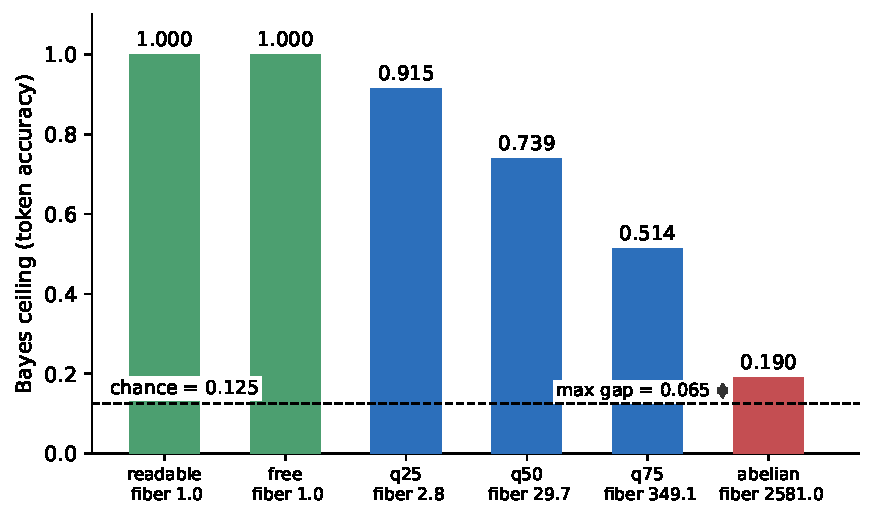
\includegraphics[width=0.85\textwidth]{figs/f5_ceilings.pdf}
\caption{The impossibility figure. Exact Bayes ceilings per condition (fiber sizes in parentheses), chance level dashed. No monotone law from fiber size to the supervision gap can pass through these bars. \emph{Source: figure created by the author from project data~\cite{appliedrepo2026}.}}
\label{fig:ceiling}
\end{figure}

The registration had also planned, as illustration, to place Parts I and III on the fitted curve after the fact. With the curve retired, the Part~I versus Part~III contrast stands as a recoverability-controlled domain difference, measured by the $0.003$ diagnostic, not as evidence for a quantitative law.

\subsection{The claim, exactly sized}

{\sloppy
For this family of operation systems, under generation-from-endpoints evaluation, \emph{no monotone law from fiber size to the supervision gap can exist}: the achievable gap is bounded by ceilings that collapse at both ends of the axis. This is a claim about this family and this evaluation mode, not a general impossibility theorem. Its provenance is the point: the quantity was defined in Lean, its consequences computed exactly in \texttt{ceiling.py}, and the conjecture it refutes was pre-registered before the computation refuted it. The standalone lesson is the pair of \texttt{readable} and \texttt{free}: identical fiber (1.0), opposite computational invertibility. Information and computation are separate axes, and the formal quantity, fiber size alone, is incomplete by construction.
\par}

\subsection{A second falsified predictor}\label{sec:secondneg}

The fiber law died of its own ceilings. A sharper candidate arrived from conversation: Sebastien Seboih conjectured a cost-function version. Attach a linear cost with nonzero coefficients on every state component, aggregated along the witness. Then endpoint data (start, end, total cost) should fail to recover the cost function where paths are ambiguous, while traces succeed. This is the right kind of conjecture: it names a quantity, a mechanism, and a predicted gap.

The test is exact linear algebra (\texttt{identifiability.py}, all $8^6$ paths per system). For each condition, build what the endpoint pair tells the regression (fiber-averaged state components and total cost) and what the trace adds, and compute the rank each side gives cost recovery (Table~\ref{tab:ident}).

\begin{table}[htbp]
\centering\footnotesize
\caption{Cost-function identifiability, exact computation over all $8^6$ paths per system. Rank of the cost-recovery regression from trace features and from endpoint (pair) features; deficit is the dimension the endpoint features cannot see. \emph{Source: project data~\cite{appliedrepo2026}.}}
\label{tab:ident}
\begin{tabular}{lcccc}
\toprule
opset & $\log_2$ fiber & rank trace & rank pair & deficit \\
\midrule
readable & 0.00 & 19 & 19 & 9 \\
free & 0.00 & 28 & 28 & 0 \\
q25 & 1.51 & 28 & 28 & 0 \\
q50 & 4.89 & 28 & 28 & 0 \\
q75 & 8.45 & 28 & 28 & 0 \\
abelian & 11.33 & 9 & 9 & 19 \\
\bottomrule
\end{tabular}
\end{table}

Two readings settle it. Wherever the dynamics are rich, the fiber-mean features span the full 28-dimensional space, so an exact endpoint learner recovers the cost completely (deficit 0). Where the deficit is nonzero (readable, abelian), it binds the trace arm identically: unexcited components are unidentifiable from any data, the persistence-of-excitation condition hiding inside the conjecture's ``nonzero coefficients'' clause. The relative trace-versus-pair deficit is zero in every system. The conjectured gap cannot occur here, and the design was stopped before registration.

One quantity survives: the finite-sample noise of the endpoint learner is the within-fiber cost variance, which here is strictly monotone in $\log$ fiber (0.0004, 0.1395, 0.2792, 0.3978, 0.5534 for free, q25, q50, q75, abelian). That suggests a variance-alone sample-complexity predictor. Direct simulation of an OLS endpoint learner falsifies it: samples to excess risk 0.05 give $n/\mathrm{variance}$ ratios of 789, 663, 654, 199 across q25, q50, q75, abelian, non-constant and direction-inverted. The highest-variance system was the easiest, because its endpoint features span only 9 of 28 dimensions.

The two-factor quantity, variance times effective rank of the endpoint features, repairs the predictor: $n\,\epsilon/(\mathrm{variance}\times\mathrm{rank})$ = 1.41, 1.18, 1.17, 1.10 across the same systems, constant within a factor of 1.3 where variance alone spans $4.0\times$ and flips sign. Sizing: for linear learners this is textbook regression theory confirmed on these systems; whether neural learners obey it is open, and Section~\ref{sec:limitations} names it as a registered open question.

The structural point: three candidate predictors entered this project through this route (the fiber, cost-function identifiability, variance-alone sample complexity), and exact computation killed all three before a single wasted training run (artifacts: \texttt{REGISTERED\_NEGATIVE.md} with its dated addenda, \texttt{identifiability.py}, \texttt{variance.py}, and \texttt{ols\_sample\_complexity.py}). A fourth survived the exact-computation filter and had to be taken to an experiment; it is Part~VI (Section~\ref{sec:part6}).

\section{Part V: The Mechanism, Tested by Budget}\label{sec:part5}

\subsection{Question and design}

Part~IV retired the information-theoretic explanation. Two mechanism candidates remain for the Part~III advantage. \emph{Data efficiency}: the pair arm never sees witness tokens in stage~1, so it must learn the witness vocabulary and distribution from stage~2 alone; enough stage-2 data should erase the difference. \emph{Structural transfer}: stage-1 trace exposure conveys something about the state-to-tactic correspondence that endpoint data cannot supply at any stage-2 budget. The registered design holds stage~1 fixed per arm and varies the stage-2 budget over $N \in \{125, 250, 500, 1000, 2000, 4000\}$, with nested draws (each smaller set a prefix of the next), so that at a given $(N, \text{seed})$ every arm sees identical examples in identical order. Registered predictions: P5a, the gap decreases with $\log_2 N$ (slope $< 0$, $p < 0.05$); P5b, at $N = 4000$ the gap is below $+0.02$ and no longer significant; P5c, the anchor: at $N = 2000$ the gap lands within $\pm 0.025$ of Part~III's $+0.054$.

Two known slack sources were stated before running, so the anchor check is distributional, not exact: Part~III drew its stage-2 set with \texttt{random.sample} while this design uses shuffle-then-prefix to keep budgets nested, and stage~1 runs as a separate process, so the random state entering stage~2 differs. A small-$N$ caveat was also stated: at $N = 125$ stage~2 is roughly four optimizer steps; all six points enter the regression regardless.

\subsection{Results}

\begin{table}[htbp]
\centering\small
\caption{Part V budget curve, seed 0. The pair arm plateaus from $N=1000$; the trace arm keeps improving to its best at $N=4000$. \emph{Source: project data~\cite{appliedrepo2026}.}}
\label{tab:budget}
\begin{tabular}{rcccc}
\toprule
$N$ & \texttt{pw\_trace} & \texttt{pw\_pair} & gap & $p$ \\
\midrule
125 & $-0.0736$ & $-0.1823$ & $+0.1086$ & $2.0\times10^{-27}$ \\
250 & $-0.0699$ & $-0.1483$ & $+0.0784$ & $3.0\times10^{-15}$ \\
500 & $-0.0715$ & $-0.1397$ & $+0.0682$ & $3.5\times10^{-11}$ \\
1000 & $-0.0573$ & $-0.1302$ & $+0.0729$ & $3.1\times10^{-14}$ \\
2000 & $-0.0718$ & $-0.1245$ & $+0.0527$ & $5.8\times10^{-9}$ \\
4000 & $-0.0427$ & $-0.1256$ & $+0.0829$ & $1.2\times10^{-13}$ \\
\bottomrule
\end{tabular}
\end{table}

\begin{figure}[htbp]
\centering
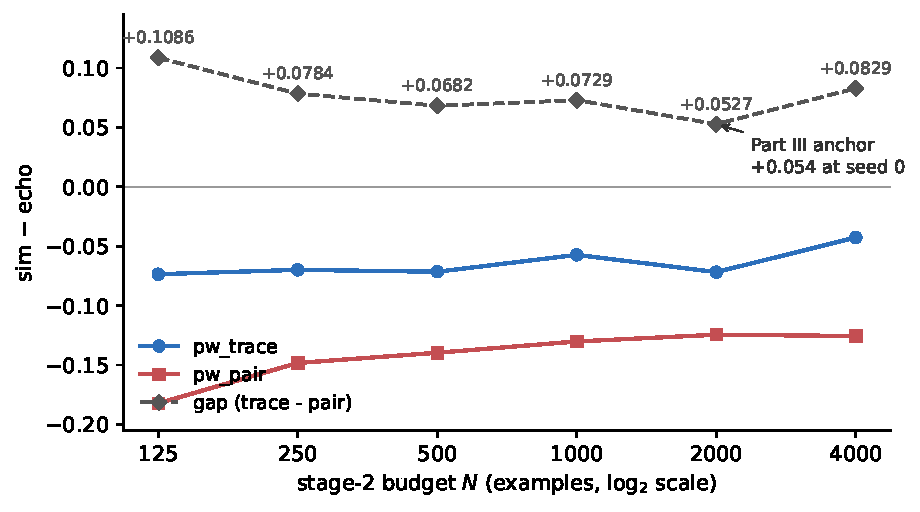
\includegraphics[width=0.9\textwidth]{figs/f4_budget_curve.pdf}
\caption{The budget curve: arm scores and the gap against the stage-2 budget on a $\log_2$ scale. The gap at $N=2000$ anchors Part~III; the gap at $N=4000$ is the largest since $N=125$. \emph{Source: figure created by the author from project data~\cite{appliedrepo2026}.}}
\label{fig:budget}
\end{figure}

Verdicts. P5c \textbf{passed}: $+0.0527$ against the $+0.054$ anchor, a miss of 0.0013. The pipeline measures what Part~III measured. P5a \textbf{failed}: slope $-0.0057$ on six points, $r^2 = 0.335$, $p = 0.229$, no significant decay. P5b \textbf{failed decisively}: at $N = 4000$ the gap is $+0.0829$, $p = 1.2\times10^{-13}$, the largest since the four-optimizer-step regime at $N = 125$. Extrapolating the flat, insignificant slope anyway gives a zero-crossing near $2^{22.9} \approx 8.0$ million examples; I report it as an extrapolation beyond the tested range, which is what it is. The pattern shows in the arm scores, not just the gap: the pair arm plateaus at $\approx -0.125$ from $N = 1000$ onward, while the trace arm keeps improving to its best score at $N = 4000$. The 4000-vs-2000 uptick ($+0.030$, $p = 0.079$) is suggestive only, and I label it as such.

\subsection{The registered conditional: decomposition at \texorpdfstring{$N = 4000$}{N = 4000}}

Because P5b failed, the pre-registered conditional took effect: train \texttt{pw\_shuffle} stage~1, fine-tune once at $N = 4000$, and decompose the surviving gap. Content (trace $-$ shuffle): $+0.0563$ (176 to 99, $p = 5.2\times10^{-6}$). Format (shuffle $-$ pair): $+0.0266$ (175 to 108, $p = 9.0\times10^{-5}$). Content share 68\%, against Part~III's 73\% at $N = 2000$ (76\% across seeds). The composition of the gain survives the budget test, not only its size.

\begin{figure}[htbp]
\centering
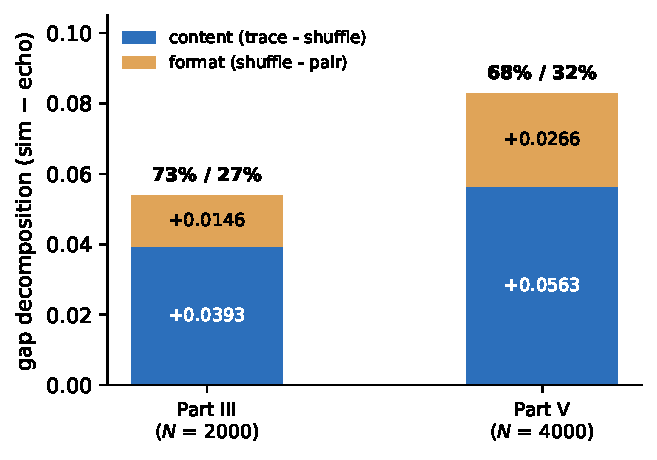
\includegraphics[width=0.47\textwidth]{figs/f6_decomposition.pdf}
\caption{Content/format decomposition at the two operating points. The content share is stable (73\% to 68\%) across a doubling of the stage-2 budget. \emph{Source: figure created by the author from project data~\cite{appliedrepo2026}.}}
\label{fig:decomp}
\end{figure}

\subsection{The final claim, exactly sized}

The trace advantage in this domain is majority witness content, is not format familiarity, and is not purchasable with endpoint fine-tuning data across a $32\times$ budget range. Two uncertainty statements belong inside the claim, not in a footnote: the curve is single-seed, and Part~III's own cross-seed magnitude swing is a factor of two. The honest statement is that the gap persists everywhere it was measured, with magnitude known only to that factor.

\section{Part VI: The Cost Channel, and What Ceilings Do Not Predict}\label{sec:part6}

\subsection{Why a third rung}

Parts~I and III are the two ends of a binary: the witness is either determined by the endpoints or it is not. Sebastien Seboih's construction supplies the rung between them. Give every operation a unique nonzero cost, sum it along the path, and keep $(\text{start}, \text{end}, \text{cost})$. Because the cost is a sum over operations, it depends only on how many times each operation occurs, never on their order. The scalar therefore reveals the operation \emph{multiset} and nothing more, which places it strictly between endpoint-only and full witness supervision. Section~\ref{sec:secondneg} reports the identifiability version of his conjecture, which exact computation falsified before any run. This section reports the version that survived to an experiment.

The design is testable precisely where Part~IV's was not. Part~IV died because its quantity vanished at both ends of its axis. The channel advantage does not: the exact Bayes ceilings (Table~\ref{tab:ccceil}, all $8^6$ witnesses enumerated per system) show the cost-channel ceiling rising \emph{faster} than the endpoint ceiling falls as fibers widen. The ceiling difference is strictly monotone in $\log_2$ fiber, Spearman $+1.00$. That difference is the maximum advantage the channel can confer, and it is largest exactly where the endpoints are least informative.

\begin{table}[htbp]
\centering\footnotesize
\caption{Exact Bayes ceilings for the cost channel, by full enumeration of all $8^6 = 262{,}144$ witnesses per system. \textsc{diff} is the maximum advantage the cost channel can confer over endpoint pairing; it is strictly monotone in $\log_2$ fiber. \emph{Source: project data~\cite{appliedrepo2026}.}}
\label{tab:ccceil}
\begin{tabular}{lccccc}
\toprule
system & $\log_2$ fiber & ceiling (pair) & ceiling (cost) & ceiling (cost+dist) & \textsc{diff} \\
\midrule
readable & 0.00 & 1.000 & 1.000 & 1.000 & 0.000 \\
free & 0.00 & 1.000 & 1.000 & 1.000 & 0.000 \\
q25 & 1.51 & 0.915 & 0.921 & 0.977 & 0.006 \\
q50 & 4.89 & 0.739 & 0.781 & 0.886 & 0.041 \\
q75 & 8.45 & 0.514 & 0.587 & 0.699 & 0.074 \\
abelian & 11.33 & 0.190 & 0.363 & 0.393 & 0.173 \\
\bottomrule
\end{tabular}
\end{table}

\subsection{Design}

Six systems, the algebra unchanged from Part~IV. One rendering change repairs Part~IV's fatal flaw: states render as hex digits rather than 28 binary characters, so the model can parse them. Under hex rendering \texttt{readable} becomes a literal copy task, which is what makes it usable as an anchor. Four arms at identical budget, single stage, examples matched: \texttt{sc\_pair} (start + end), \texttt{sc\_cost} (start + end + cost), \texttt{sc\_costd} (adds the running distance-to-goal sum, an order-\emph{sensitive} term), and \texttt{sc\_counts} (the same action information spelled out as eight per-operation counts). Costs are powers of seven, verified collision-free over all six-draw multisets, so the scalar determines the multiset exactly.

The \texttt{sc\_cost}/\texttt{sc\_counts} pair is the instrument that makes the result interpretable: the two arms carry \emph{identical information} and differ only in how much arithmetic it takes to read. Model Pythia-160M, fp32, seed 0, 30{,}000 witnesses per system, metric token accuracy over the six operation slots against a chance level of $0.125$. The witness alphabet is disjoint from the state alphabet, so copying cannot beat chance. Twenty-four runs.

Registered predictions. A1, the anchor: all arms $\geq 0.90$ on \texttt{readable}, with an explicit abort rule if it fails. A2, accessibility: on \texttt{abelian}, \texttt{sc\_counts} exceeds \texttt{sc\_pair} by $\geq 0.05$, without which C1 is untestable. C1, primary: the measured advantage is positively rank-correlated with the ceiling difference. C2: \texttt{sc\_counts} minus \texttt{sc\_cost}, the decoding cost of identical information, no direction committed. C3: the order term is largest in the middle systems and smaller at \texttt{abelian} than at \texttt{q75} --- a non-monotone shape predicted from the ceilings, because for commuting flips the distance to the goal is the same in every order, so the order-sensitive term goes order-blind exactly where order is the only remaining unknown.

The registered falsification clause: if C1 fails while A1 and A2 both pass, then models do not extract available information in proportion to how much is present, and the ceiling table does not predict learned behavior.

\subsection{Results: the clause fired}

\begin{table}[htbp]
\centering\footnotesize
\caption{Part VI, measured token accuracy by system and arm (seed 0, $n=300$ held out). The advantage the cost channel actually confers runs \emph{opposite} to the advantage it could confer. \emph{Source: project data~\cite{appliedrepo2026}.}}
\label{tab:ccmain}
\begin{tabular}{lcccccc}
\toprule
system & \texttt{sc\_pair} & \texttt{sc\_cost} & \texttt{sc\_costd} & \texttt{sc\_counts} & cost $-$ pair & ceiling \textsc{diff} \\
\midrule
readable & 1.000 & 1.000 & 1.000 & 1.000 & $+0.000$ & 0.000 \\
free & 0.183 & 0.348 & 0.331 & 0.341 & $+0.166$ & 0.000 \\
q25 & 0.143 & 0.319 & 0.351 & 0.329 & $+0.176$ & 0.006 \\
q50 & 0.201 & 0.301 & 0.363 & 0.301 & $+0.100$ & 0.041 \\
q75 & 0.249 & 0.300 & 0.362 & 0.297 & $+0.051$ & 0.074 \\
abelian & 0.185 & 0.257 & 0.268 & 0.256 & $+0.073$ & 0.173 \\
\bottomrule
\end{tabular}
\end{table}

A1 \textbf{passed}: all four arms at $1.0000$ on \texttt{readable} against the $0.90$ bar, so the hex rendering repairs Part~IV's failure mode and the pipeline can measure. A2 \textbf{passed}: \texttt{abelian} counts $-$ pair $= +0.0716$ against the $0.05$ bar, so the model can use fully explicit multiset information where the ceiling difference is largest.

C1 \textbf{failed, in the registered direction of falsification}. Measured advantages run $+0.166$, $+0.176$, $+0.100$, $+0.051$, $+0.073$ across free, q25, q50, q75, abelian, against ceiling differences of $0.000$, $0.006$, $0.041$, $0.074$, $0.173$: Spearman $\rho = -0.80$, and \texttt{abelian} does not exceed \texttt{free} but sits $0.093$ below it. With both anchors passing, the falsification clause fires as written. The cost channel helps everywhere, and least where it should help most.

C2 is \textbf{null everywhere} --- \texttt{sc\_counts} and \texttt{sc\_cost} differ by at most $0.011$ in absolute value across all systems --- and that null is what makes the C1 failure interpretable. The aggregate scalar is as accessible to the model as the spelled-out counts, so the failure is not an arithmetic-reading artifact: the information was present, legible, and demonstrably usable, and the model still did not use it in proportion to how much there was.

C3 \textbf{confirmed}. The order term (\texttt{costd} $-$ \texttt{cost}) measures $+0.032$, $+0.062$, $+0.062$, $+0.011$ across q25, q50, q75, abelian: largest in the middle, smaller at \texttt{abelian} than at \texttt{q75}, matching the ceiling analysis ($+0.056$, $+0.105$, $+0.112$, $+0.029$) in shape at roughly half magnitude. The one prediction in this experiment derived from exact structure rather than from an information count is the one that held.

\subsection{The search evaluation}

A registered addendum tests the construction's intended use: fix the endpoints, ask the cost-conditioned model for progressively cheaper paths, and verify each candidate by running it forward. Generation is unreliable and verification is cheap, so invalid candidates are discarded rather than trusted --- return-conditioned generation with a soundness guarantee bolted on. Only costs \emph{achievable} for that endpoint pair are requested, enumerated exactly, so a miss means the model failed rather than that the request was impossible. The ladder per item is the true cost, the median achievable cost, the minimum achievable cost, and one value below the minimum as an impossible control.

R1, the control, \textbf{passed}: the impossible rung scores $0.000$ valid-and-cost-matching in all three searchable systems, so the models read the cost field and the rest of the table is interpretable. R2 \textbf{passed} in all three. R3, the primary number with no threshold committed, is $0.102$ (q50), $0.380$ (q75), $0.783$ (abelian) at the minimum-cost rung. R4 \textbf{passed}: that ordering follows the co-optimal path counts ($1.59$, $3.25$, $296.3$ mean minima), so uniqueness \emph{failure} helps the search --- more distinct valid targets, easier hits.

That last point has a consequence worth stating plainly. Exact computation shows the fraction of endpoint pairs with a unique minimum-cost path falls from $100\%$ (free) to $0.8\%$ (abelian), with 296 co-optimal paths on average in the commuting case. Existence of an optimal path is trivial; uniqueness fails structurally wherever operations commute, because any reordering of a minimum-cost path is another minimum-cost path to the same endpoint. Quantum gate sets commute extensively, so an existence-and-uniqueness result for optimal circuits should be expected to fail on the uniqueness half for exactly this reason. One post-hoc note, not a registered check: on \texttt{abelian} the minimum rung ($0.783$) sits below both true ($0.944$) and median ($0.972$), the documented non-extrapolation signature of return conditioning --- muted here, but present.

\subsection{What this part adds}

Part~IV showed that an information-theoretic quantity can be falsified by its own exact consequences before any model is trained. Part~VI is the sharper case, because here the quantity survived that test. Its ceilings are monotone, its ceiling difference is largest exactly where endpoint supervision is weakest, and the accessibility anchor confirms the model can use the information when it is spelled out. The prediction still failed, and failed with a negative rank correlation rather than a flat one.

The claim, exactly sized: for this family and this evaluation, available information does not predict used information, and a correct ceiling calculation is not a forecast of learned behavior. Three of the four predictors this project registered were killed by exact computation before training; this is the one that had to be killed by the experiment. Sizing the negative honestly, it is single-seed, one model scale, and synthetic --- the same limitations Part~IV carries, and they bound this conclusion the same way.

\section{Synthesis}\label{sec:synthesis}

\begin{table}[htbp]
\centering\small
\caption{The whole result in one table. Recoverability, not fiber size, separates the domains; the mechanism evidence comes from the controls, not the headlines.}
\label{tab:synthesis}
\begin{tabular}{llll}
\toprule
domain & witness recoverable? & supervision gap & mechanism evidence \\
\midrule
code diffs & yes (determined) & null ($p = 0.152$) & n/a (echo-repaired) \\
proof steps & 0.003 verbatim & $+0.024$ to $+0.050$ & 68 to 76\% content; not buyable (Part~V) \\
\bottomrule
\end{tabular}
\end{table}

The honest general statement: where the record of a computation is recoverable from its endpoints, supervising on it adds nothing measurable. Where recovery is search, trace supervision transfers something that endpoint data does not supply at any budget tested, and most of what transfers is content, not format. The non-claims are part of the result, listed rather than implied: nothing here bears on P versus NP; the fiber is falsified as the predictor of when trace supervision pays, and the correct predictor is open; larger models are untested; the hardware result is one device, one calibration era, one registered seed.

\section{Methods, Rigor, and Disclosure}\label{sec:methods}

\paragraph{Pre-registration ledger.} I registered fifteen protocols as timestamped commits to the project repository before the corresponding runs, and recorded verdicts against them before interpretation. Two registered designs (R1, R2) are reported as confounded alongside their corrected reruns.

\begin{table}[htbp]
\centering\scriptsize
\caption{Pre-registration ledger. Short hashes refer to the project repository~\cite{appliedrepo2026}.}
\label{tab:prereg}
\begin{tabular}{@{}lll >{\raggedright\arraybackslash}p{5.2cm}@{}}
\toprule
protocol & registered (UTC) & commit & verdict status \\
\midrule
Part I: edit-witness P1 to P4 & 2026-07-18 & \texttt{89da3fc} & complete; v1 metric error repaired \\
Part II: hardware ladder + control & 2026-07-18 & \texttt{89da3fc} & direction confirmed; ordering falsified \\
Part III: P1/P2/P3 & 2026-07-24 & \texttt{dc3dcaa} & P1 confirmed; P2 falsified \\
Part III addendum: shuffle C1/C2 & 2026-07-24 & \texttt{930b2b2} & C1 confirmed; C2 observed positive \\
Mirror M1 to M3 (hardware witness) & 2026-07-24 & \texttt{59a1385} & M3 confirmed; M2 failed low on all four \\
Round 2 R1 (DD mirror) & 2026-07-24 & \texttt{671ac0d} & confounded (cross-job); rerun as R1$'$ \\
Round 2 R2 (seed-11 rerun) & 2026-07-24 & \texttt{671ac0d} & confounded (layout); rerun as R2$'$ \\
Round 2 R3 (Part III multi-seed) & 2026-07-24 & \texttt{671ac0d} & R3a/b/c all confirmed \\
Round 3 R1$'$ (drift-controlled DD) & 2026-07-24 & \texttt{563edcd} & DD uniformly harmful; dephasing rejected \\
Round 3 R2$'$ (matched layout) & 2026-07-24 & \texttt{563edcd} & R2$'$a/b/c all confirmed \\
Part IV: fiber law P4a to P4d & 2026-07-24 & \texttt{75f0e4c} & P4c failed; design retired by exact ceilings \\
Part V: budget curve P5a to P5c + cond. & 2026-07-25 & \texttt{ae895f7} & P5c passed; P5a/b failed; conditional ran \\
Verification V0$'$ to V5 (dissociation) & 2026-07-26 & \texttt{7c7f87b} & V0$'$ passed; V1 failed twice (masked retry); closed uninterpretable \\
Cost-function registered negative & 2026-07-26 & \texttt{2ead38e} & identifiability falsified; variance-alone falsified in addendum \\
Cost-channel experiment (intermediate rung) & 2026-07-26 & \texttt{7058507} & A1/A2 passed; C1 falsified as registered; search R1--R4 passed \\
\bottomrule
\end{tabular}
\end{table}

\paragraph{Verification and reproduction.} \texttt{verify.py} runs 39 checks and re-derives every table in this paper from committed artifacts~\cite{appliedrepo2026}: pair equality from the committed QASM, transpile identity against the recorded runs, aer reproduction, hardware-delta significance, ceiling saturation, and the Part~I statistics from per-item scores. Every part reruns from the repository root with the committed scripts, smoke-tested on CPU first as registered. The reader is invited to run it.

\paragraph{Tool disclosure, specific.} Lean proof search across the broader formal program used Aristotle (Harmonic). Claude (Anthropic) contributed engineering scaffolding, analysis drafting, and the initial drafts of the error-budget analysis, \texttt{verify.py}, the recoverability formalization, the ceiling derivation, and the identifiability and sample-complexity computations. Every experimental design decision, every verdict call against the pre-registrations, and every sentence of prose in this paper is mine. I rederived by hand: the two faithfulness proofs, the ceiling bound, the error-budget computation, and the OLS excess-risk scaling argument. Where this paper states a result, I can defend the derivation. The bias throughout is to underclaim rather than overclaim.

\paragraph{Data and code availability.} All experiments, pre-registrations, raw JSON artifacts, and \texttt{verify.py} are public in the project repository~\cite{appliedrepo2026}. The formal mathematics behind the ZX rewrite rules is developed in the companion Lean repositories~\cite{liquidtqft2026}: 12{,}777 lines across 33 files, no proof placeholders, no custom axioms, machine-checked against Mathlib v4.28.0~\cite{mathlib2020,demoura2021lean}.

\section{Limitations and Future Work}\label{sec:limitations}

One quantum device and one calibration era. One model scale, 160M parameters. A single-seed budget curve with a factor-of-two cross-seed magnitude uncertainty. The metric-blindness hypothesis for the mirror undershoot remains untested, labeled rather than carried. Registered hardware follow-ups, in order of information per dollar: the transpile-seed sweep on \texttt{mod\_mult\_55} (done, Section~\ref{sec:part2}); a second device on a different day, to test whether the ordering scrambles identically; optimization level 3, to test whether the vendor transpiler equalizes the arms, which is itself a finding; and the mirror protocol at larger package sizes.

\paragraph{The verification experiment, run and closed.} Parts I to V measure whether trace supervision helps \emph{generation}; the registered follow-up asked whether it helps \emph{checking}, a dissociation test (search versus checking) on the Part~III stems: 598 balanced instances, five negative strata, labels audited by hand (tallies 0/15, 1/15, 1/15, 0/8, 0/8; two flagged negatives dropped). It stopped at its own anchor twice. V1 required every arm at $\geq 0.90$ on the surface stratum; unmasked training gave 0.860 / 0.581 / 0.860 (trace / pair / shuffle) with an always-no lean (VALID 0.53 to 0.66), and the registered masked-loss retry gave 0.581 / 0.605 / 0.512 with the opposite lean (VALID 0.75 to 0.92). One diagnostic pattern is worth reporting: under masking, the after-swap stratum hit 1.000 in two arms (0.992 in the third) while all tactic-swap strata sat near chance, so the models judged state-pair coherence and ignored the tactic, the shortcut the fifth stratum existed to expose. The only supported claim is one sentence: at 160M parameters and these budgets, tactic-level witness verification does not get off the ground, so the search/checking dissociation remains open.

Two questions are registered as open, each requiring a new registration: the search/checking dissociation, and the two-factor (variance $\times$ rank) predictor for neural learners. Sebastien Seboih is the source of both threads. His third thread was registered, run, and closed: the cost-channel ceiling table did not predict learned usage, and the full report is in the repository~\cite{appliedrepo2026}.

\section*{Acknowledgments}

I thank Sebastien Seboih for the cost-function conjecture of Section~\ref{sec:secondneg} and for the search-versus-checking framing that Section~\ref{sec:limitations} closes.


{\singlespacing
\bibliography{refs}
}

\end{document}
